\begin{frame}[noframenumbering,plain]

\begin{tikzpicture}[remember picture,overlay]
\fill[blue1]
(current page.north west) rectangle ([xshift=-12.cm,yshift=-10.cm]current page.east|-{pic cs:end});
\end{tikzpicture}

\begin{textblock}{0.22}(0.02,0.06)
	
\includegraphics[width=\textwidth]{Sources/title/Logo_FAU_DinA4_RGB_Negativ.png}
%		\vspace{2cm}
	
\includegraphics[width=\textwidth]{Sources/title/mss_negative.png}
	\vspace{1.5cm}
\end{textblock}
\begin{textblock}{0.25}(0.05,0.45)
	\textcolor{white}{
	{\large PhD defense \\
		\textbf{Manuel Baur}}}
\end{textblock}

\begin{textblock}{0.23}(0.01,0.7)
	\centering
	\begin{spacing}{.9}
		\textcolor{white}{
		\footnotesize{
			{\setstretch{.1}
			Funded by the German Federal Ministry for Economic Affairs and Energy,
			grant no.\ 50WM 1653}
			}
		}
	\end{spacing}
\end{textblock}



% make title
\begin{textblock}{0.65}(0.3,0.05)
	\begin{center}
		\textcolor{blue1}{							
		\Large{\textbf{
			X-ray radiography of granular systems\\
			-- particle densities and dynamics}}
		}
	\end{center}
\end{textblock}


\begin{textblock}{0.4}(0.3,0.25)
	\centering
	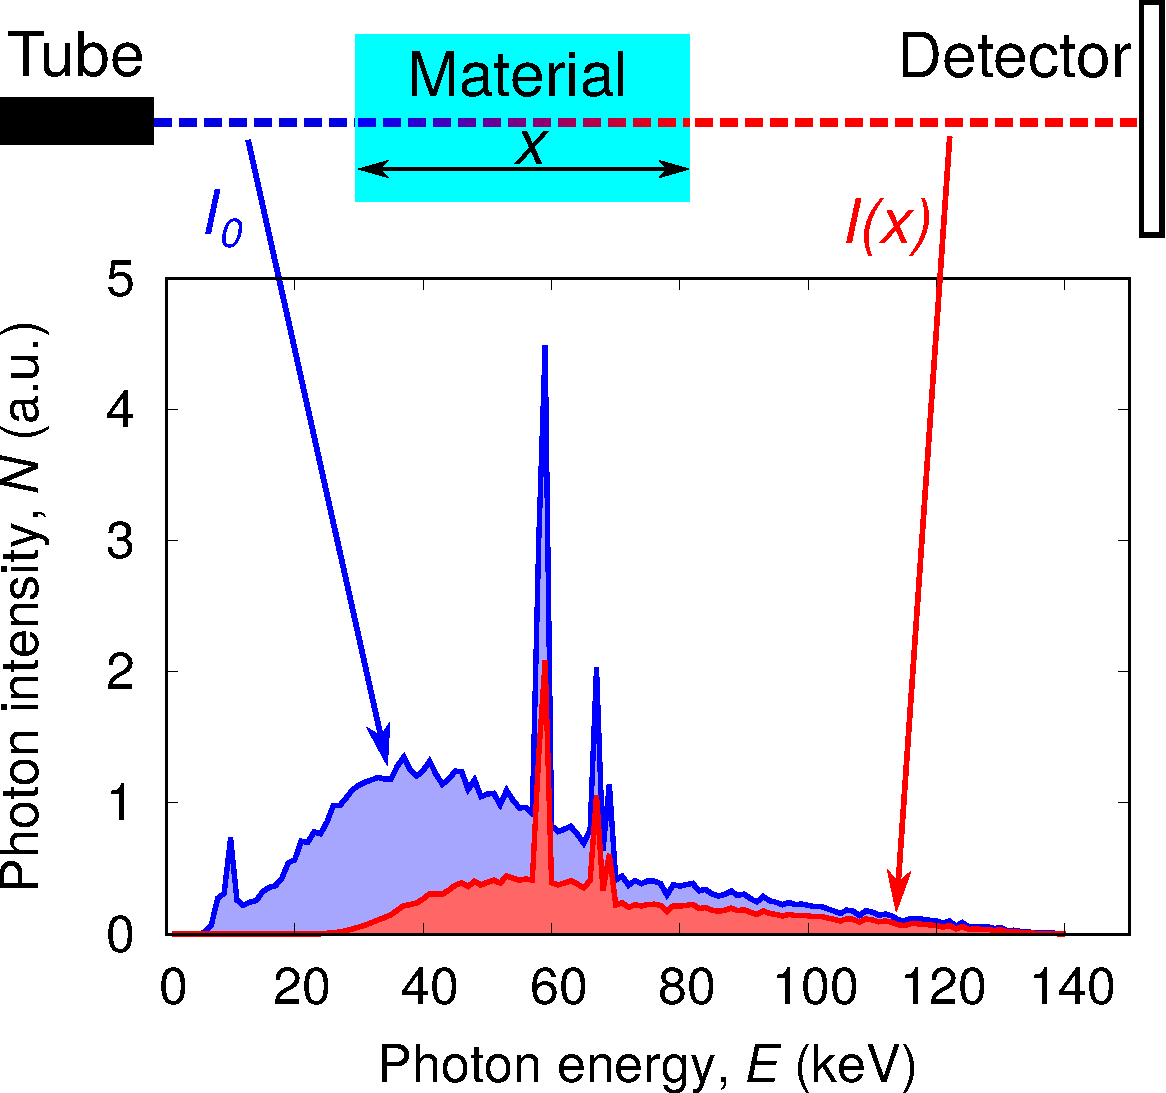
\includegraphics[width=\textwidth]
	{Sources/beam_hardening/x-ray_spectra_beam_hardening.pdf}
\end{textblock}
	
\begin{textblock}{0.25}(0.72,0.35)
	\centering
	\centering
	\movie[width =\textwidth, poster, loop]
	{
\includegraphics[width=\textwidth]{Sources/X-DFA/cropped_80kV_340uA_38ms_0000.png}}
	{videos/fluidized_3500mul_per_min.avi}
\end{textblock}

\end{frame}


